
%\section{TDNN}
\label{sec:application:tdnn}

For the implementation of the two kinds of dynamic ANNs already
described,
\ie, the TDNN (\subsecref{ANN:TDNN}) and the NARX models (\subsecref{ANN:NARX}), 
we also made used of the MatLab Toolbox for neural networks. 

Since we can consider a TDNN as a NARX model with the same input TDL
and a null delayed connection from the output to the input layer, the
bulding process of both ANNs is practically equal. Hence, if the
previous values of the independent exogenous input signal $u(t)$ in
the NARX model was denoted as $d_{u}$, we can express the same way the
TDL time steps of the TDNN. For simplicity during the ANNs
implementation, we denote this parameter as $n_{b}$. The delayed
connection from the output to the input layer ($d_{y}$ in the NARX
model), if exists, is from now expressed as $n_{a}$.  Finally, the
prediction horizon is denoted as $n_{k}$ as it happens with the
feedforward networks (\subsecref{perceptronapplication}).

The most paramount aspect we must take into account is that samples
cannot be introduced in the dynamic network the same way as with a
static one.  In the latter, all the samples of a entire time-window
are presented to the network at a time, that is, samples are
concurrent.  In dynamic networks, only one sample of each time series
is introduced every step, maintaining always the temporal order among
samples. Therefore we must indicate the Toolbox that the network
inputs are sequencial signals and not concurrent samples. With MatLab,
this process is carried out using the cell format instead of the
matrix one. Notice that also de output must be defined as a sequential
signal.

The turn of the screw is in the fact that we have a set of four
concurrent physiological time series. Therefore, we must combine the
matrix and the cell format in order to point out that samples are
sequential within their corresponding signal, but concurrent with the
samples of the same time step of the other physiological time series.

The following sections expose the peculiarities and results of the
Time Delay and NARX networks used.



%%%%%%%%%%%%%%%%%%%%%%%%%%%%%%%%%%%%%%%%%%%%%%%%%%
%%%%%%%%%%%%%%%%%%%%%%%%%%%%%%%%%%%%%%%%%%%%%%%%%%
\subsection{TDNN}
\label{subsec:tdnnapplication}

\figref{tdnnbuilt} shows an example of a TDNN built.
\begin{figure}[!ht]
\centering
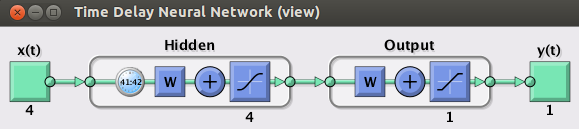
\includegraphics[width=0.9\columnwidth]{images/results/tdnn}
\caption{Example of a TDNN we have evaluated}
\label{fig:tdnnbuilt}
\end{figure}

From left to right, we can observe that it comprises a set of four input concurrent samples, 
one for each physiological signal (HR, EDA, TEMP, SpO2). This signals are formatted as sequencial in order to preserve its temporal characteristic.

The circle we found next represents the TDL and usually consists on two numbers. The first one determines the prediction horizon $n_{k}=(41)-1=40$ (it is substracted $1$ because MatLab enumerates the time steps starting by $1$). The difference between the second number and the first one fixes the amount of input previous values used to compute the output, \ie, the memory of the system. Therefore, $n_{b}=(42-41)+1=2$ (it is added $1$ because the ends of the interval are also taken into account).

Both $n_{k}$ and $n_{b}$, as well as the number of physiological signals used, are modified and evaluated. Thus, we set the next experimental ranges: $n_{k}\in [10,40]$, $n_{b}\in [1,5]$. Greater values of $n_{k}$ improves the prediction, while if $n_{b}$ increases, more memory and computation capacities requires the ANN.

We observed that there are four neurons in the hidden layer -in fact, we configured the network to have the number of hidden neurons equals to the amount of physiological signals in the input layer. All of them have an hyperbolic tangent sigmoid as activation function. On the contrary, the unique output neuron has a symetric saturating linear function. These types of transfer function have been set after experimenting several alternatives. None of the layers have biases terms.

Althought the training phase presents an acceptable outcome (\figref{tdnntraining}), the test phase is always much worse (\figref{tdnntest}). This difference can be an evidence of overfitting of the training set, which is very common when the number of well-known patterns are ver low.

\begin{figure}[!ht]
\centering
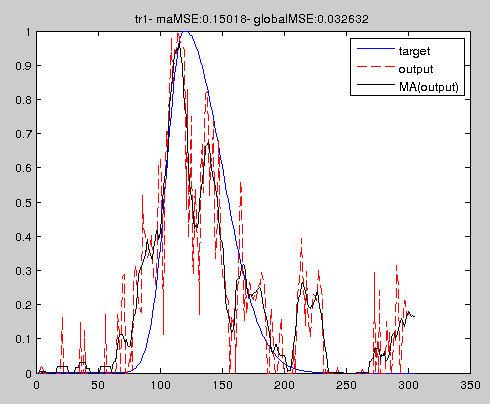
\includegraphics[width=0.7\columnwidth]{images/results/tdnnTraining}
\caption{Acceptable outcome of a TDNN while training}
\label{fig:tdnntraining}
\end{figure}

\begin{figure}[!ht]
\centering
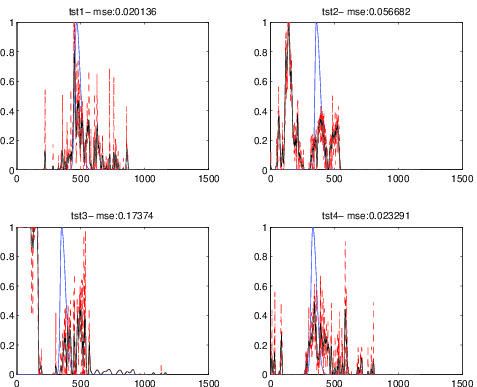
\includegraphics[width=0.9\columnwidth]{images/results/tdnnTest}
\caption{Non acceptable result of a TDNN in the test phase}
\label{fig:tdnntest}
\end{figure}

Notice that the original output of the network (red) is almost chaotic, but performing its 12-points moving average (MA), a more target-alike signal (blue) is obtained. However, with this test results, it is hard to set a threshold value with which conclude that a migraine is detected in advanced.



%%%%%%%%%%%%%%%%%%%%%%%%%%%%%%%%%%%%%%%%%%%%%%%%%%
%%%%%%%%%%%%%%%%%%%%%%%%%%%%%%%%%%%%%%%%%%%%%%%%%%
\subsection{NARX}
\label{subsec:narxapplication}

As done with the other topologies, we configure the NARX ANN for a maximum of four exogenous inputs, the four physiological signals of our experimental scenario. 
For that purpose, it can be observed in \figref{narxopenloop} that the example of NARX is almost identical to the example of the above TDNN (\figref{tdnnbuilt}). 

The only difference is the $y(t)$ term, in the input layer, with its corresponding delay and weight. This term corresponds to the previous values of the output signal $d_{y}$ (\eref{narxequation}), but we express it from now as $n_{a}$.  In fact, in order to reduce complexity, it is always set to $n_{b}$, \ie, equals to the the amount of input previous values used to compute the output.


\begin{figure}[!ht]
\centering
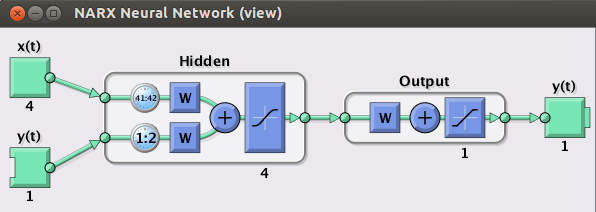
\includegraphics[width=0.9\columnwidth]{images/results/narxOpenloop}
\caption{Example of an open-loop NARX network we have evaluated}
\label{fig:narxopenloop}
\end{figure}

Notice that the $y(t)$ is the output of the entire network. 
However, the input term does not appear as a feedback of the output. 
The reason is that \figref{narxopenloop} depictes an open-loop NARX network, which corresponds to the series-parallel architecture of \figref{narxtrainingarch}. 
As we exposed in \subsecref{ANN:NARX}, this topology is well accepted for the training phase. 
Then, 
The NARX network is converted to the close-loop configuration for validating and 
testing the model. An example of a close-loop NARX can be see in \figref{narxcloseloop}.
\begin{figure}[!ht]
\centering
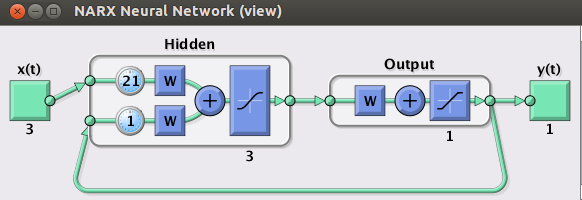
\includegraphics[width=0.9\columnwidth]{images/results/narxCloseloop}
\caption{The close-loop NARX network we have obtained the best test results with}
\label{fig:narxcloseloop}
\end{figure}

It is exactly this latter topology the one with the best results of prediction we have obtained. They are depicted in \figref{narxTest}.
\begin{figure}
\centering
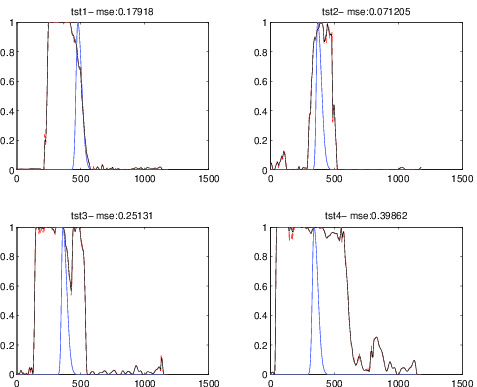
\includegraphics[width=\columnwidth]{images/results/trn3_na-nb1-nk20_NN3}
\caption{NARX model test for the four migraines considered}
\label{fig:narxTest}
\end{figure}


We can observe that the output curve (red/black) does not adjust to the target one (blue) -the performance metric (MSE) results written in the title of each graphic can corroborate this lack of fitting. However, the four migraines can be detected by thresholding the output. The clue is that the output curve must reach the threshold value before (or at the same time in the worst case) as the real migraine -target- does. If the contrary occurs, then the algorithm will fail and  the pain will begin before the system can notify the patient that a headache is arriving.

What is drawn in \figref{narxTest} is therefore a great result, since the network output is always ahead in time, so the prediction is possible in all cases. 
As we will expose later, the NARX network that produces these outcomes were trained with a forecasting horizon of $n_{k}=20$ . 
However, we can notice that, in \figref{narxTest}, the prediction can be anticipated until some hundreds of minutes before, always depending on the value of the threshold. 

This lvariable margin of prediction has one great advantage and an important inconvenient. 
It has in favour that, the earlier the migraine can be predicted, the more effective pharmacological treatment can be administrated.
The disadvantage is the fact of not be capable of notifying the patient when the headache is going exactly to arrive.

Turning to the threshold, its determination is a function of the admissible porcentage of false-positive and false-negative predictions. 
Hence, we rise the value of the threshold whether false positives are wanted to be avoid. 
Inversely, the amount of false-negative forecastings can be decreased if the threshold value falls too.
Then, the ``reset'' threshold must be set in a way that little output falls during the migraine detection such as the one shown in the bottom-left graphic of \figref{narxTest}, do not produce a too early reset process.

The following lines listed in detail the configuration process of the NARX network
in order to allow an exact reproduction of the ANN.

\subsubsection{Configuration}

\begin{description}
\item {\textbf{About the neural network}\hfill \\
\begin{tabular}{p{5cm}l}
 	topology: &``narxnet''\\
    neuronsInHidden: &3\\
    layHiddenTransFnc: &``tansig''\\
    layOutTransFnc: &``satlins''\\
    weightsInitFnc: &``rands''\\
    layHiddenBias: &0\\
    layOutBias: &0\\
\end{tabular}
}

\item {\textbf{About the AR model}\hfill \\
\begin{tabular}{p{5cm}l}
    $n_{b}$: &1 \\
    $n_{k}$: &20 \\
    $n_{a}$: &1 
\end{tabular}
}

\item {\textbf{About the training phase}\hfill \\
Only truncated time series are considered for the training. The interval of time used for this phase is defined has its bottom edge in (BegOfAura-NsamplesWinBeforeAura) and its upper edge in  (BegOfPain+NsamplesWinAfterPainBegins).\\
\begin{tabular}{p{5cm}l}
	NsamplesWinBeforeAura: &120 \\
    NsamplesWinAfterPainBegins: &60 \\
    NretrainedNN: &5 \\
    epochs: &100
\end{tabular}
}

\item {\textbf{About the input and output data}\hfill \\
\begin{tabular}{p{5cm}l}
	preprocess: &``data 60 gpml noise added''\\
   numOuts: &1\\
    parserSignals: &``norm''\\
  parserTarget: &``standardGauss2''\\
    sources: &``HR, TEMP, SPO2''
\end{tabular}

where ``data 60 gpml noise  added'' means that the sampling frequency is $1/(60 \text{seconds}$ and input data have been first preprocessed with a Gaussian Process Machine Learning (GPML) in order to recover disruptions \cite{Rasmussen06gaussianprocesses} and then added some noise.
Besides, the input signals are normalised in the range of $[0,1]$. Then, ``standardGauss2'' denotes the process for building the target curve as described in \secref{paincurve}. Finally, the order in which the sources are listed is crutial. 
}

\item {\textbf{About the test phase}\hfill \\
Inputs weights, where each row index corresponds to an input neuron and each column index denotes a different physiological signal:\\
\begin{center}
\begin{tabular}{ c c c }
    0.0631   & 0.0830   & 0.0554 \\
    0.1298   & 0.2843   & 0.1116 \\
    0.0933   &-1.4993   & 0.2123
\end{tabular}
\end{center}

Output feedback weigths:
\begin{center}
\begin{tabular}{ c c c }
	3.5602  & -1.9144   &-0.1467
\end{tabular}
\end{center}
}

Hidden to output weights:
\begin{center}
\begin{tabular}{ c }
0.0972\\
   -0.4118\\
    0.7611
    \end{tabular}
\end{center}

\end{description}

